Building upon the foundational concepts introduced in the previous
section, this section delves deeper into the technical intricacies of
the Bitcoin protocol. We will begin by exploring Bitcoin Script, the
simple yet powerful scripting language that underpins all Bitcoin
transactions. We will examine how this stack-based language is used to
create sophisticated spending conditions, enabling a wide range of
transaction types beyond simple payments.

The section will then trace the evolution of Bitcoin's standard script
types, from the early Pay-to-Public-Key (P2PK) and
Pay-to-Public-Key-Hash (P2PKH) scripts to the more advanced
Pay-to-Script-Hash (P2SH) and multi-signature (P2MS) scripts. We will
analyze the motivation behind each of these developments and the new
capabilities they introduced.

A significant portion of this section is dedicated to the two most
important upgrades in Bitcoin's history: Segregated Witness (SegWit) and
Taproot. We will explore the technical details of these upgrades,
including how SegWit solved the long-standing problem of transaction
malleability and how Taproot introduced Schnorr signatures and
Merkelized Alternative Script Trees (MAST) to enhance privacy,
efficiency, and smart contract capabilities.

%\ih{drop} Finally, we will discuss the concept of blockchain forks in greater
%detail, examining the different types of forks and their implications
%for the network. We will also analyze the threat of a 51\% attack and
%other potential vulnerabilities that could compromise the security and
%integrity of the Bitcoin network.

\subsection{Learning Objectives}\label{learning-objectives}

\begin{itemize}
	\tightlist
	\item
	Understand the fundamentals of Bitcoin Script and its role in defining
	spending conditions.
	\item
	Learn about the different standard script types, including P2PK,
	P2PKH, P2SH, and the various SegWit and Taproot formats.
	\item
	Grasp the concepts of transaction malleability and how Segregated
	Witness (SegWit) addresses this issue.
	\item
	Understand the benefits of the Taproot upgrade, including improved
	privacy and efficiency.
%	\item
%	\ih{drop} Learn about the different types of blockchain forks and their
%	implications for the network.
	\item
	Gain insight into the 51\% attack and other potential vulnerabilities
	in the Bitcoin network.
\end{itemize}

\begin{center}\rule{0.5\linewidth}{0.5pt}\end{center}

\subsection{The UTXO Model and Bitcoin
	Script}\label{section-1-the-utxo-model-and-bitcoin-script}

\subsubsection{Recap of the UTXO
	Model}\label{recap-of-the-utxo-model}

As established in the preceding section, the Bitcoin protocol employs
the \textbf{Unspent Transaction Output (UTXO)} model as its fundamental
accounting mechanism. This model represents a paradigm shift from the
traditional account-based systems used in conventional finance. Instead
of maintaining balances in accounts, the Bitcoin ledger comprises a
collection of UTXOs, each representing a discrete and unspent amount of
bitcoins. Every transaction consumes one or more UTXOs as inputs and
generates one or more new UTXOs as outputs, thereby creating a
continuous and verifiable chain of ownership.

\subsubsection{Introduction to Bitcoin
	Script}\label{introduction-to-bitcoin-script}

At the heart of the UTXO model is \textbf{Bitcoin Script}, a simple,
stack-based programming language that governs the spending conditions
for each UTXO. Every transaction output is encumbered with a locking
script, formally known as \texttt{ScriptPubKey}, which specifies the
conditions that must be met to spend the associated funds. To redeem a
UTXO, a subsequent transaction must provide a corresponding unlocking
script, or \texttt{ScriptSig}, that satisfies the requirements of the
\texttt{ScriptPubKey} (see \autoref{fig:utxo-unlock}).


\begin{figure}[t]
	%	\vspace{-0.3cm}
	\begin{center}
		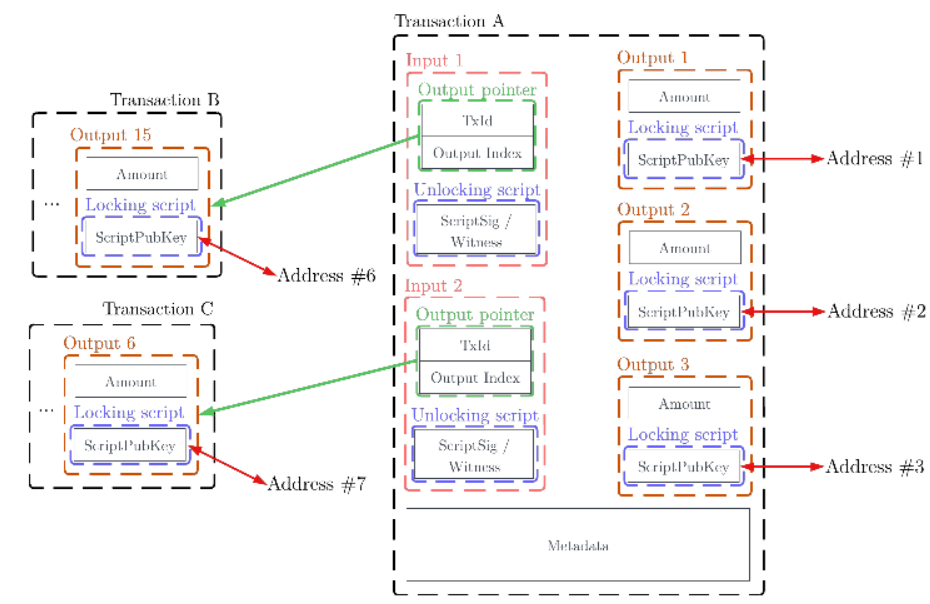
\includegraphics[width=0.9\textwidth]{./figs/utxo-unlocking.png}
		\caption{Bitcoin transaction with locking and unlocking scripts.}		
		\label{fig:utxo-unlock}
	\end{center}	
\end{figure}



The design of Bitcoin Script is intentionally minimalistic. It is not
Turing-complete, meaning that it lacks the ability to perform loops or
complex recursive operations. This limitation is a deliberate security
feature, designed to prevent the execution of overly complex or
malicious scripts that could potentially disrupt the network.

\subsubsection{Standard Script Types}\label{standard-script-types}

While Bitcoin Script allows for a high degree of flexibility in defining
spending conditions, a set of standard script types has emerged over
time to accommodate the most common use cases. These standard scripts
are recognized and relayed by all nodes in the network, ensuring a high
degree of interoperability.

\begin{itemize}
	\item
	\textbf{Pay-to-Public-Key (P2PK)}: This was the original script type
	used in the earliest days of Bitcoin. It locks a UTXO directly to a
	specific public key, and the corresponding unlocking script simply
	requires a valid signature from the owner of that public key. While
	simple, P2PK has been largely superseded by more advanced script
	types.
	\item
	\textbf{Pay-to-Public-Key-Hash (P2PKH)}: This is the most common
	script type in use today. Instead of locking a UTXO to a public key,
	it locks it to the hash of a public key. This provides two main
	advantages: it results in a shorter and more convenient address
	format, and it offers a degree of privacy protection, as the public key is not revealed until the UTXO is spent.
	\item
	\textbf{Pay-to-MultiSig (P2MS)}: This script type enables
	multi-signature transactions, which require the approval of multiple
	parties to spend a UTXO. A P2MS script specifies a set of \texttt{n}
	public keys and a threshold \texttt{m}, where
	$m \leq n$. To spend the UTXO, at least \texttt{m}
	valid signatures corresponding to the specified public keys must be
	provided.
	\item
	\textbf{Pay-to-Script-Hash (P2SH)}: This is a more advanced and
	flexible script type that allows a UTXO to be locked to the hash of an
	arbitrary script. This enables the creation of complex spending
	conditions without revealing the underlying script until the UTXO is
	spent. P2SH is commonly used for multi-signature wallets and other
	advanced smart contract-like functionality.
\end{itemize}

\begin{center}\rule{0.5\linewidth}{0.5pt}\end{center}

\subsection{Segregated Witness (SegWit) and
	Taproot}\label{section-2-segregated-witness-segwit-and-taproot}

\subsubsection{The Need for Upgrades}\label{the-need-for-upgrades}

As the Bitcoin network grew and evolved, several limitations of the
original protocol became apparent: 

\begin{itemize}
	\tightlist
	\item
	\textbf{Transaction Malleability}: This was a long-standing
	vulnerability in the Bitcoin protocol that allowed a third party to
	alter the signature data of an unconfirmed transaction, thereby
	changing its transaction ID (TXID) without invalidating the
	transaction itself. This could cause problems for services that relied
	on unconfirmed transactions, such as payment processors and exchanges. \ih{check it}
	\item
	\textbf{Scalability}: The 1 MB block size limit severely restricted
	the number of transactions that could be processed by the network,
	leading to congestion and high fees during periods of high demand.
	\item
	\textbf{Privacy}: The public nature of the blockchain made it possible
	to analyze transaction patterns and link addresses to real-world
	identities, raising privacy concerns for users.
\end{itemize}
These challenges prompted the
development of two major upgrades: Segregated Witness (SegWit) and
Taproot \ih{refs on BIPs}. 

\subsubsection{Segregated Witness
	(SegWit)}\label{segregated-witness-segwit}

Segregated Witness (SegWit) was a soft fork upgrade that was activated
on the Bitcoin network in August 2017. It addressed the issue of
transaction malleability by separating the \textbf{signature data}, or
``\textbf{witness},'' from the main transaction data. By moving the witness data to a separate data structure, SegWit made it impossible for a third
party to alter the signature and change the TXID.

In addition to fixing transaction malleability, SegWit also introduced a
new concept of ``block weight,'' which effectively increased the block
size limit to 4 MB for blocks containing SegWit transactions. This
allowed for more transactions to be included in each block, thereby
improving the scalability of the network.

SegWit also introduced new address formats, known as \textbf{P2WPKH
(Pay-to-Witness-Public-Key-Hash)} and \textbf{P2WSH (Pay-to-Witness-Script-Hash)},
which offer lower transaction fees than their legacy counterparts. To
ensure backward compatibility, SegWit also provided a mechanism for
``wrapping'' SegWit transactions in P2SH addresses.
Overview of all existing output types in UTXO is depicted in \autoref{fig:btc-scripts}.

\begin{table}[t]
	%	\vspace{-0.3cm}
	\begin{center}
		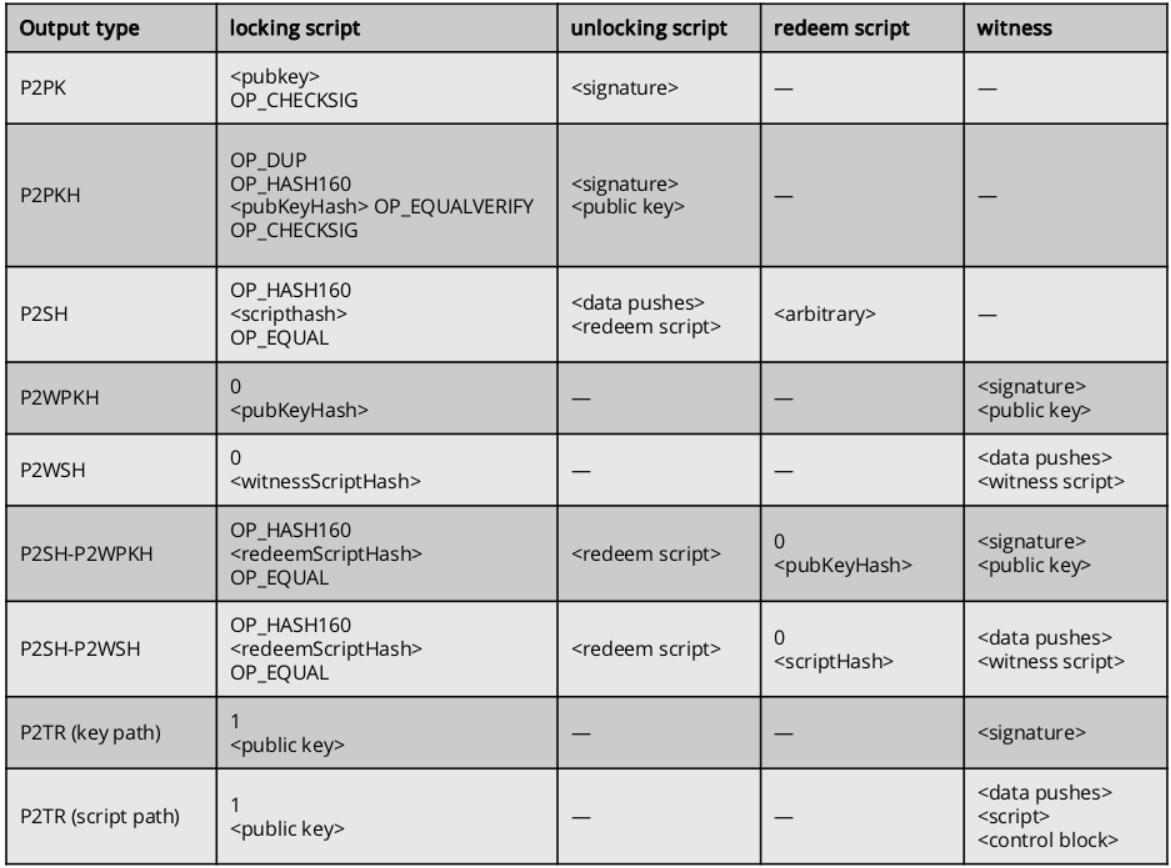
\includegraphics[width=0.9\textwidth]{./figs/scripts}
		\caption{Output types in UTXO and their locking and unlocking scripts.}		
		\label{fig:btc-scripts}
	\end{center}	
\end{table}

\subsubsection{Taproot}\label{taproot}

Taproot is the most significant upgrade to the Bitcoin protocol since
SegWit, and it was activated in November 2021. It introduced a number of
new features that further enhance the privacy, efficiency, and smart
contract capabilities of the network. I  particular, Taproot introduced the following:

\begin{itemize}
	\item
	\textbf{Schnorr Signatures}: Taproot replaced the Elliptic Curve
	Digital Signature Algorithm (ECDSA) with Schnorr signatures. Schnorr
	signatures offer several advantages over ECDSA, including their
	smaller size and their ability to be aggregated. This means that
	multiple signatures can be combined into a single signature, which
	makes multi-signature transactions indistinguishable from
	single-signature transactions on the blockchain. This significantly
	improves the privacy of multi-signature wallets and reduces their
	transaction fees since only one signature is enough to be stored.
	\item
	\textbf{MAST (Merkelized Alternative Script Trees)}: Taproot also
	introduced Merkelized Alternative Script Trees (MAST), a new way of
	constructing complex spending conditions. With MAST, a user can create
	a tree of different scripts, each representing a different spending
	condition. When the UTXO is spent, only the script that is actually
	used is revealed on the blockchain. This improves privacy by hiding
	the other possible spending conditions, and it also reduces the amount
	of data that needs to be stored on the blockchain, thereby improving
	efficiency.
\end{itemize}

\subsubsection{Ordinals and
	Inscriptions}\label{ordinals-and-inscriptions}

The Taproot upgrade had an unforeseen consequence: the emergence of
\textbf{Ordinals and Inscriptions}. The Ordinals protocol is a system
for numbering individual satoshis\ih{check this}, the smallest unit of bitcoin, and
tracking them across transactions. The Inscriptions protocol allows
users to inscribe arbitrary data, such as images and text, onto
individual satoshis.

This has led to the creation of NFT-like assets on the Bitcoin
blockchain, which has been a source of considerable controversy within
the community. While some see it as an innovative new use case for
Bitcoin, others are concerned that it is leading to network congestion
and higher transaction fees, and that it is a departure from Bitcoin's
original purpose as a peer-to-peer electronic cash system.

\begin{center}\rule{0.5\linewidth}{0.5pt}\end{center}

\subsection{The 51\% Attack}\label{section-3-blockchain-forks-and-network-security}

A 51\% attack is a potential attack on a Proof-of-Work blockchain where
a single entity or a group of colluding entities gains control of more
than 50\% of the network's total mining hash rate. With this level of
control, an attacker could theoretically:

\begin{itemize}
	\tightlist
	\item
	\textbf{Prevent new transactions from being confirmed}: By refusing to
	include certain transactions in the blocks they mine, an attacker
	could effectively censor users.
	\item
	\textbf{Halt payments between some or all users}: By creating empty
	blocks, an attacker could prevent any transactions from being
	processed.
	\item
	\textbf{Reverse transactions}: An attacker could use their majority
	hash power to create a private chain that is longer than the public
	chain. They could then broadcast this longer chain to the network,
	which would cause the public chain to be orphaned and all the
	transactions in it to be reversed. This would allow the attacker to
	double-spend their coins.
\end{itemize}

While a 51\% attack is a serious threat, it is important to note that it
is extremely difficult and expensive to execute on a large and
decentralized network like Bitcoin. The cost of acquiring the necessary
hardware and electricity to control more than 50\% of the Bitcoin
network's hash rate would be astronomical. Furthermore, a successful
51\% attack would likely undermine confidence in the network, causing
the price of the cryptocurrency to plummet and rendering the attack
unprofitable.

\begin{center}\rule{0.5\linewidth}{0.5pt}\end{center}

\subsection{Summary / Key Takeaways}\label{summary-key-takeaways}

This section has provided a deep dive into the advanced technical
aspects of the Bitcoin protocol, building upon the foundational
knowledge from the previous section. We have explored the evolution of
Bitcoin's scripting capabilities, from the simple yet powerful Bitcoin
Script to the sophisticated features introduced by the SegWit and
Taproot upgrades.

We have examined the various standard script types, including P2PK,
P2PKH, P2MS, and P2SH, and we have seen how they enable a wide range of
transaction types. We have also analyzed the motivations behind the
SegWit and Taproot upgrades, and we have seen how they have addressed
key challenges such as transaction malleability, scalability, and
privacy.

\begin{center}\rule{0.5\linewidth}{0.5pt}\end{center}

\subsection{Keywords}\label{keywords}

\begin{itemize}
	\tightlist
	\item
	\textbf{Bitcoin Script}: A simple, stack-based programming language
	that is used to define the conditions under which a UTXO can be spent.
	\item
	\textbf{Segregated Witness (SegWit)}: A protocol upgrade that
	addresses transaction malleability and increases the effective block
	size by separating the signature data from the main transaction data.
	\item
	\textbf{Taproot}: A protocol upgrade that enhances privacy,
	efficiency, and smart contract capabilities through the introduction
	of Schnorr signatures and Merkelized Alternative Script Trees (MAST).
	\item
	\textbf{Blockchain Fork}: A divergence in the blockchain that results
	in two or more competing chains.
	\item
	\textbf{51\% Attack}: A potential attack on a Proof-of-Work blockchain
	where a single entity controls more than 50\% of the network's mining
	hash rate.
	\item
	\textbf{P2PKH (Pay-to-Public-Key-Hash)}: The most common type of
	Bitcoin transaction, where the output is locked to the hash of a
	public key.
	\item
	\textbf{P2SH (Pay-to-Script-Hash)}: A type of Bitcoin transaction that
	allows for more complex spending conditions by locking the output to
	the hash of a script.
	\item
	\textbf{Schnorr Signatures}: A digital signature scheme that is more
	efficient and secure than ECDSA and allows for key and signature
	aggregation.
	\item
	\textbf{MAST (Merkelized Alternative Script Trees)}: A mechanism that
	allows for more complex and flexible smart contracts by enabling the
	creation of a tree of possible spending conditions.
	\item
	\textbf{Ordinals and Inscriptions}: A protocol that allows for the
	creation of NFT-like assets on the Bitcoin blockchain.
\end{itemize}

\begin{center}\rule{0.5\linewidth}{0.5pt}\end{center}

\subsection{Further Reading}\label{further-reading}

\begin{itemize}
	\tightlist
	\item
	\textbf{Bitcoin Improvement Proposals (BIPs)}:\\
	\url{https://github.com/bitcoin/bips}
	\item
	\textbf{Learn Me a Bitcoin}: \\ 
	\url{https://learnmeabitcoin.com/}
	\item
	\textbf{Mempool.space}: \\
	\url{https://mempool.space/}
\end{itemize}